\section{Simple model}
We start with the simplest form of this problem. With a fixed number of people waiting to be tested, when does it take fewer total tests if the samples are pooled and tested together first. Since $p$ is the infection rate , the probability of not infected will be $(1-p)$.
\subsection{Two samples}
For testing 2 samples in ideal solution, we consider the following possibilities:

\begin{itemize}
  \item For all the samples negative. The probability is $(1-p)^2$. Only 1 test is required.
  \item For 1 of the samples positive, 1 of the samples negative. The probability is $p(1-p)$. 3 tests is required. But if the first sample is tested negative, only 2 test is required as the last sample must be positive.
  \item For all the samples positive. The probability is $p^2$. 3 tests is required.
\end{itemize}
Similarly, the expected number of test:
\\
\begin{displaymath}
t(p)=3p^2+(1-p)^2+2(1-p)p+3p(1-p)
\end{displaymath}
\\
Simplifying $t(p)$, we get:
\\
\begin{displaymath}
t(p)=-p^2+3p+1
\end{displaymath}
\\
For solving $t(p)=2$, we get:
\\
\begin{center}
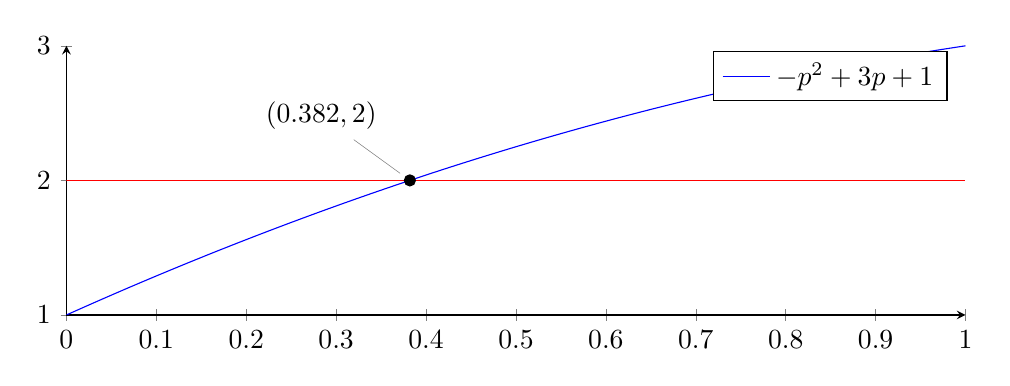
\begin{tikzpicture}
\begin{axis}[
    axis lines = left,
    ytick={0,1,2,3},
    xtick={0,0.1,0.2,0.3,0.4,0.5,0.6,0.7,0.8,0.9,1},
    height=5cm,
    width=13cm,
]

\addplot [
    domain=0:1, 
    samples=1000, 
    color=blue,
    ]
    {-x^2 + 3*x + 1};
\addlegendentry{\(-p^2+3p+1\)}

\addplot [
    domain=0:1, 
    samples=100, 
    color=red,
    ]
    {2};
    
\addplot[mark=*] coordinates {(0.382,2)} node[pin=120:{$(0.382,2)$}]{} ;

\end{axis}
\end{tikzpicture}
\end{center}
\\
From the graph, we find that when the group size is equal to 2, pooling should be used only when $p<0.382$ such that the expected amount of tests used is lower than the traditional way.

\subsection*{Worse Case of Two Samples}
If the first grouping test is positive, the samples had to be retested individually. From the method above, we considered a special case of testing: If all of the samples tested before the last one got a negative result, we assume that the last sample must be positive. But in reality, the samples may not be tested one by one but simultaneously. Which means that this special case may not exist in reality, for example, in a sample of 2, for 1 of the samples positive, 1 of the samples negative.  The probability is $p(1 -− p)$. The case for only 2 test is required as the last sample must be positive will not be considered, such that there will only be neither 1 test or 3 tests used in every group.
\\
\\
Similar to the ideal 2 sample test, we consider the following possibilities:

\begin{itemize}
  \item For all the samples negative. The probability is $(1-p)^2$. Only 1 test is required.
  \item For 1 of the samples positive, 1 of the samples negative. The probability is $p(1-p)$. 3 tests is required. 
  \item For all the samples positive. The probability is $p^2$. 2 tests is required.
\end{itemize}
The new expected number of test will be given out by:
\\
\begin{displaymath}
T(p)=3p^2 + 3p(1-p) \times 2 + 1(1-p)^2
\end{displaymath}
\\
Simplifying $T(p)$, we get:
\\
\begin{displaymath}
T(p)=-2p^2+4p+1
\end{displaymath}
\\
For solving $T(p)=2$, we get:
\\
\begin{center}
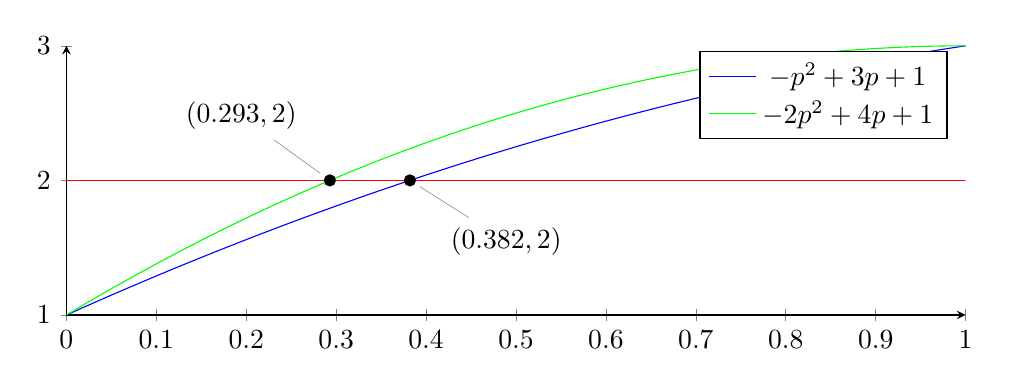
\begin{tikzpicture}
\begin{axis}[
    axis lines = left,
    ytick={0,1,2,3},
    xtick={0,0.1,0.2,0.3,0.4,0.5,0.6,0.7,0.8,0.9,1},
    height=5cm,
    width=13cm,
]

%Here the blue parabola is defined
\addplot [
    domain=-0:1, 
    samples=100, 
    color=blue,
    ]
    {-x^2 + 3*x + 1};
\addlegendentry{\(-p^2+3p+1\)}

%Here the red parabola is defined
\addplot [
    domain=0:1, 
    samples=100, 
    color=green,
    ]
    {-2*x^2 + 4*x + 1};
\addlegendentry{\(-2p^2+4p+1\)}

%Here y=2 is defined
\addplot [
    domain=0:1, 
    samples=100, 
    color=red,
    ]
    {2};

%Two dots are defined
\addplot[mark=*] coordinates {(0.293,2)} node[pin=120:{$(0.293,2)$}]{} ;
\addplot[mark=*] coordinates {(0.382,2)} node[pin=310:{$(0.382,2)$}]{} ;

\end{axis}
\end{tikzpicture}
\end{center}
\\
From the graph, we find that in the worse case, when the group size is equal to 2, pooling should be used only when $p<0.293$ such that the expected amount of tests used is lower than the traditional way.
\\
\\
We can compare the two expected functions by considering the difference:
\\
\begin{displaymath}
D(p)=T(p)-t(p)=-2p^2+4p+1-(-p^2+3p+1)
\end{displaymath}
\\
Solving $D(p):$
\\
\begin{displaymath}
D(p)=-p^2+p
\end{displaymath}
\\
The difference of the two equations is a cubic equation.
\\
\\
Graphing the equation:
\\
\begin{center}
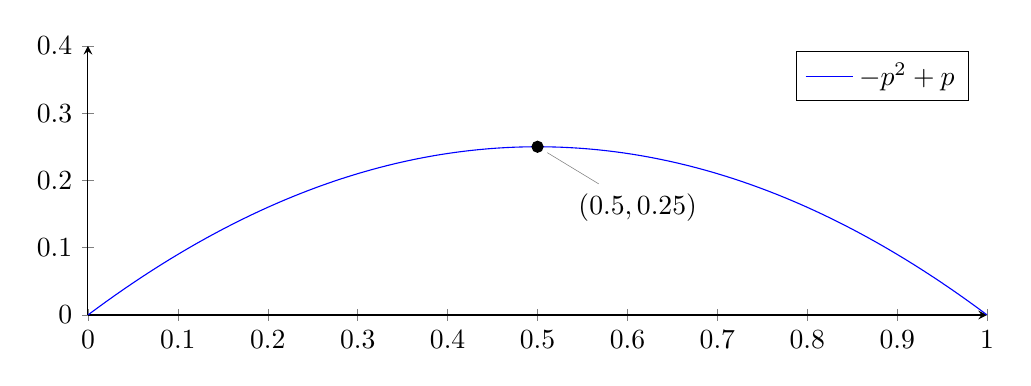
\begin{tikzpicture}
\begin{axis}[
    axis lines = left,
    ytick={0,0.1,0.2,0.3,0.4},
    ymin=0.0,ymax=0.4,
    xtick={0,0.1,0.2,0.3,0.4,0.5,0.6,0.7,0.8,0.9,1},
    height=5cm,
    width=13cm,
]

%Here the blue parabola is defined
\addplot [
    domain=0:1, 
    samples=100, 
    color=blue,
    ]
    {-x^2 +x};
\addlegendentry{\(-p^2+p\)}

%Two dots are defined
\addplot[mark=*] coordinates {(0.5,0.25)} node[pin=310:{$(0.5,0.25)$}]{} ;

\end{axis}
\end{tikzpicture}
\end{center}
\\
From the graph, we noticed that the vertex of the equation is $(0.5,0.25)$, which means that the biggest difference occurs when $p=0.5$ and the expected value of the two models differ by 0.25 tests.
\subsection{Three samples}
For testing 3 samples in ideal solution, we consider the following possibilities:

\begin{itemize}
  \item For all the samples negative. The probability is $(1-p)^3$. Only 1 test is required.
  \item For 1 of the samples positive, 2 of the samples negative. The probability is $p(1-p)^2$. 4 tests is required. But if the first 2 samples are tested negative, only 3 test is required as the last sample must be positive.
  \item For all the samples positive. The probability is $p^3$. 4 tests is required.
  \item For 2 of the samples positive, 1 negative. The probability is $p^2(1-p)$.  4 tests is required.
\end{itemize}
The expected number of test:
\\
\begin{displaymath}
t(p)=4p^{3}+1(1-p)^{3}+4p^{2}(1-p) \times 3+4p(1-p)^{2} \times 2+3p(1-p)^{2}
\end{displaymath}
\\
Simplifying $t(p)$, we get:
\\
\begin{displaymath}
t(p)=2p^{3}-7p^{2}+8p+1
\end{displaymath}
\\
For solving $t(p)=3$:

\begin{center}
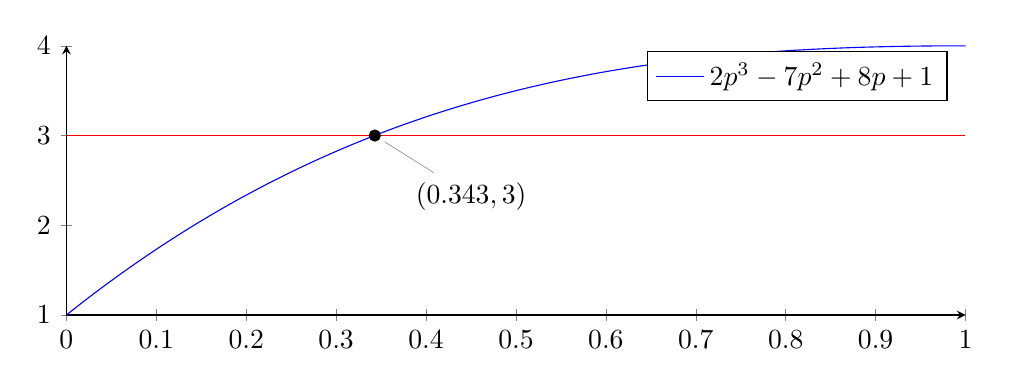
\begin{tikzpicture}
\begin{axis}[
    axis lines = left,
    ytick={0,1,2,3,4},
    xtick={0,0.1,0.2,0.3,0.4,0.5,0.6,0.7,0.8,0.9,1},
    height=5cm,
    width=13cm,
]

\addplot [
    domain=0:1, 
    samples=1000, 
    color=blue,
    ]
    {2*x^3 - 7*x^2 + 8*x + 1};
\addlegendentry{\(2p^{3}-7p^{2}+8p+1\)}

\addplot [
    domain=0:1, 
    samples=100, 
    color=red,
    ]
    {3};
    
\addplot[mark=*] coordinates {(0.343,3)} node[pin=310:{$(0.343,3)$}]{} ;

\end{axis}
\end{tikzpicture}
\end{center}
\\
From the graph, we find that when the group size is equal to 3, pooling should be used only when $p<0.343$ such that the expected amount of tests used is lower than the traditional way.

\subsection*{Worse Case of Three Samples}
\\
\\
Similar to the ideal 3 sample test, we consider the following possibilities:

\begin{itemize}
  \item For all the samples negative. The probability is $(1-p)^3$. Only 1 test is required.
  \item For 1 of the samples positive, 2 of the samples negative. The probability is $p(1-p)^2$. 4 tests is required.
  \item For all the samples positive. The probability is $p^3$. 4 tests is required.
  \item For 2 of the samples positive, 1 negative. The probability is $p^2(1-p)$.  4 tests is required.
\end{itemize}
The new expected number of test will be given out by:
\\
\begin{displaymath}
T(p)=4p^{3}+4p^{2}(1-p) \times 3+4p(1-p)^{2} \times 3 +1(1-p)^{3}
\end{displaymath}
\\
Simplifying $T(p)$, we get:
\\
\begin{displaymath}
T(p)=3p^3-9p^2+9p+1
\end{displaymath}
\\
For solving $T(p)=3$, we get:
\\
\begin{center}
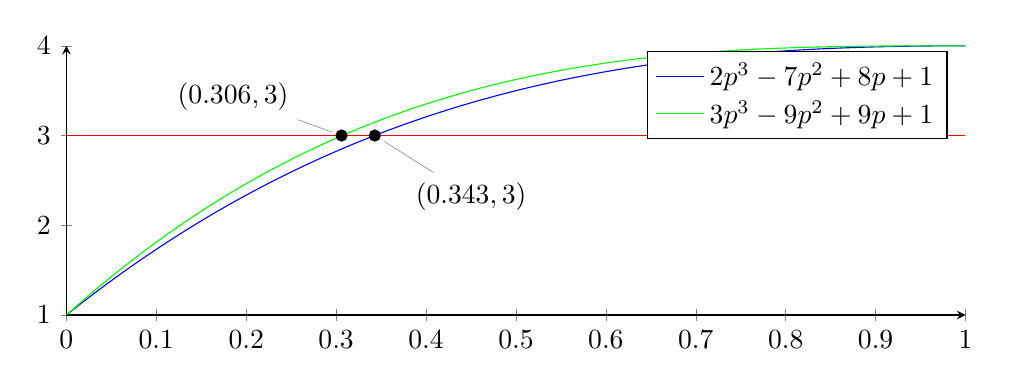
\begin{tikzpicture}
\begin{axis}[
    axis lines = left,
    ytick={1,2,3,4,5},
    xtick={0,0.1,0.2,0.3,0.4,0.5,0.6,0.7,0.8,0.9,1},
    height=5cm,
    width=13cm,
]

\addplot [
    domain=0:1, 
    samples=1000, 
    color=blue,
    ]
    {2*x^3 - 7*x^2 + 8*x + 1};
\addlegendentry{\(2p^{3}-7p^{2}+8p+1\)}

\addplot [
    domain=-0:1, 
    samples=100, 
    color=green,
    ]
    {3*x^3 - 9*x^2 + 9*x + 1};
\addlegendentry{\(3p^3-9p^2+9p+1\)}

\addplot [
    domain=0:1, 
    samples=100, 
    color=red,
    ]
    {3};

\addplot[mark=*] coordinates {(0.306,3)} node[pin=160:{$(0.306,3)$}]{} ;
\addplot[mark=*] coordinates {(0.343,3)} node[pin=310:{$(0.343,3)$}]{} ;

\end{axis}
\end{tikzpicture}
\end{center}
\\
From the graph, we find that in the worse case, when the group size is equal to 3, pooling should be used only when $p<0.306$ such that the expected amount of tests used is lower than the traditional way.
\\
\\
We can compare the two expected functions by considering the difference:
\\
\begin{displaymath}
D(p)=T(p)-t(p)=3p^3-9p^2+9p+1-(2p^{3}-7p^{2}+8p+1)
\end{displaymath}
\\
Solving $D(p):$
\\
\begin{displaymath}
D(p)=-p^2+p
\end{displaymath}
\\
The difference of the two equations is a quadratic equation.
\\
\\
Graphing the equation:
\\
\begin{center}
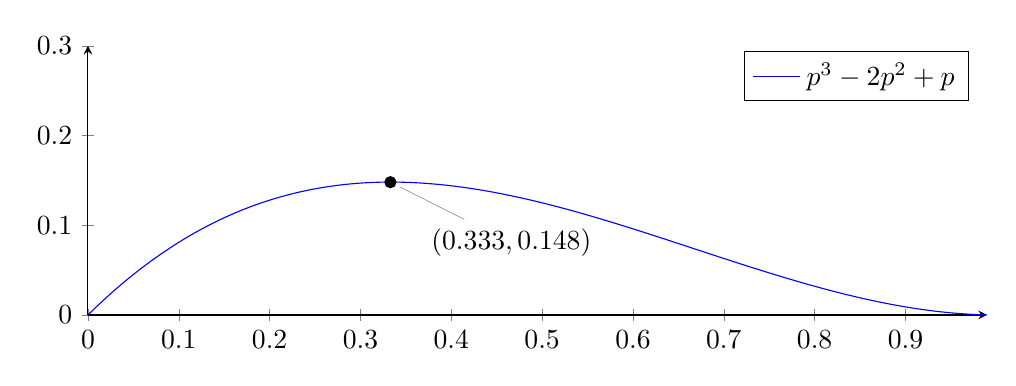
\begin{tikzpicture}
\begin{axis}[
    axis lines = left,
    ytick={0,0.1,0.2,0.3},
    ymin=0.0,ymax=0.3,
    xtick={0,0.1,0.2,0.3,0.4,0.5,0.6,0.7,0.8,0.9,1},
    height=5cm,
    width=13cm,
]

%Here the blue parabola is defined
\addplot [
    domain=0:1, 
    samples=100, 
    color=blue,
    ]
    {x^3 -2*x^2 +x};
\addlegendentry{\(p^3 -2p^2+p\)}

%Two dots are defined
\addplot[mark=*] coordinates {(0.333,0.148)} node[pin=310:{$(0.333,0.148)$}]{} ;

\end{axis}
\end{tikzpicture}
\end{center}
\\
From the graph, we can see that the vertex of the equation is $(0.333,0.148)$, which means that the biggest difference occurs when $p=0.333$ and the expected value of the two models differ by 0.148 tests.
\subsection{Four samples}
For testing 4 samples in ideal solution, we consider the following possibilities:

\begin{itemize}
  \item For all the samples negative. The probability is $(1-p)^4$. Only 1 test is required.
  \item For 1 of the samples positive, 3 of the samples negative. The probability is $p(1-p)^3$. 5 tests is required. But if the first three samples are tested negative, only 4 test is required as the last sample must be positive.
  \item For all the samples positive. The probability is $p^4$. 5 tests is required.
  \item For 3 of the samples positive and 1 negative. The probability is $p^3(1-p)$.  5 tests is required.
  \item For 2 of the samples positive, 2 negative. The probability is $p^2(1-p)^2$.  5 tests is required.
  \item For all the samples positive. The probability is $(1-p)^4$. 5 tests is required. 
\end{itemize}
Similarly, the expected number of test:
\\
\begin{displaymath}
Q(p)=5p^{4}+5p^{3}(1-p) \times 4+5 p^{2}(1-p)^{2} \times 6+5p(1-p)^{3} \times 3+4p(1-p)^{3}+1(1-p)^{4}
\end{displaymath}
\\
Simplifying $Q(p)$, we get:
\\
\begin{displaymath}
Q(p)=-3p^{4}+13p^{3}-21p^{2}+15p+1
\end{displaymath}
\\
For solving $Q(p)=4$:
\begin{center}
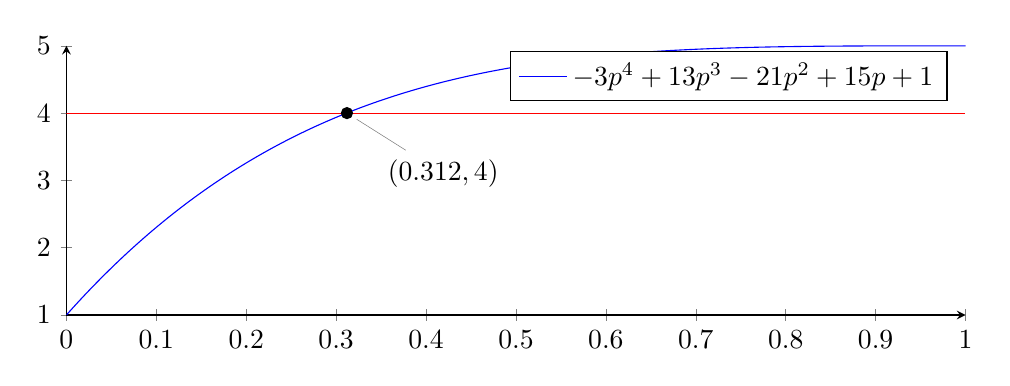
\begin{tikzpicture}
\begin{axis}[
    axis lines = left,
    ytick={1,2,3,4,5},
    xtick={0,0.1,0.2,0.3,0.4,0.5,0.6,0.7,0.8,0.9,1},
    height=5cm,
    width=13cm
]

\addplot [
    domain=0:1, 
    samples=1000, 
    color=blue,
    ]
    {-3*x^4 + 13*x^3 - 21*x^2 + 15*x + 1};
\addlegendentry{\(-3p^{4}+13p^{3}-21p^{2}+15p+1\)}

\addplot [
    domain=0:1, 
    samples=100, 
    color=red,
    ]
    {4};
\addplot[mark=*] coordinates {(0.312,4)} node[pin=310:{$(0.312,4)$}]{} ;

\end{axis}
\end{tikzpicture}
\end{center}
\\
From the graph, we find that when the group size is equal to 4, pooling should be used only when $p<0.312$ such that the expected amount of tests used is lower than the traditional way.

\subsection*{Worse Case of Four Samples}
\\
\\
Similar to the ideal 4 sample test, we consider the following possibilities:

\begin{itemize}
  \item For all the samples negative. The probability is $(1-p)^4$. Only 1 test is required.
  \item For 1 of the samples positive, 3 of the samples negative. The probability is $p(1-p)^3$. 5 tests is required.
  \item For all the samples positive. The probability is $p^4$. 5 tests is required.
  \item For 3 of the samples positive and 1 negative. The probability is $p^3(1-p)$.  5 tests is required.
  \item For 2 of the samples positive, 2 negative. The probability is $p^2(1-p)^2$.  5 tests is required.
  \item For all the samples positive. The probability is $(1-p)^4$. 5 tests is required. 
\end{itemize}
The new expected number of test will be given out by:
\\
\begin{displaymath}
T(p)=5p^{4}+5p^{3}(1-p) \times 4+5 p^{2}(1-p)^{2} \times 6+5p(1-p)^{3} \times 4+1(1-p)^{4}
\end{displaymath}
\\
Simplifying $T(p)$, we get:
\\
\begin{displaymath}
T(p)=-4p^4+16p^3-24p^2+16p+1
\end{displaymath}
\\
For solving $T(p)=3$, we get:
\\
\begin{center}
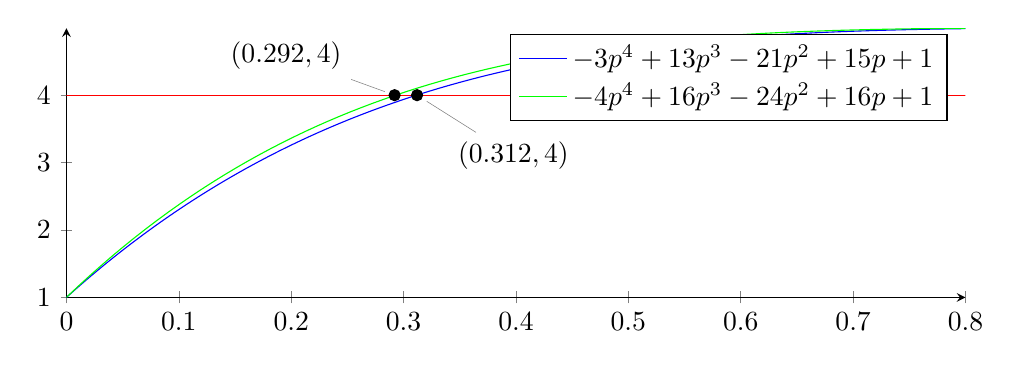
\begin{tikzpicture}
\begin{axis}[
    axis lines = left,
    ytick={1,2,3,4,5},
    xmin=0.0,xmax=0.8,
    xtick={0,0.1,0.2,0.3,0.4,0.5,0.6,0.7,0.8},
    height=5cm,
    width=13cm,
]

\addplot [
    domain=0:1, 
    samples=1000, 
    color=blue,
    ]
    {-3*x^4 + 13*x^3 - 21*x^2 + 15*x + 1};
\addlegendentry{\(-3p^{4}+13p^{3}-21p^{2}+15p+1\)}

\addplot [
    domain=-0:1, 
    samples=100, 
    color=green,
    ]
    {-4*x^4+16*x^3-24*x^2+16*x+1};
\addlegendentry{\(-4p^4+16p^3-24p^2+16p+1\)}

\addplot [
    domain=0:1, 
    samples=100, 
    color=red,
    ]
    {4};

\addplot[mark=*] coordinates {(0.292,4)} node[pin=160:{$(0.292,4)$}]{} ;
\addplot[mark=*] coordinates {(0.312,4)} node[pin=310:{$(0.312,4)$}]{} ;

\end{axis}
\end{tikzpicture}
\end{center}
\\
From the graph, we find that in the worse case, when the group size is equal to 3, pooling should be used only when $p<0.292$ such that the expected amount of tests used is lower than the traditional way. Also, we noticed that the range of  p $(p<)$ is as same as when sample equals to 2.
\\
\\
We can compare the two expected functions by considering the difference:
\\
\begin{displaymath}
D(p)=T(p)-t(p)=-4p^4+16p^3-24p^2+16p+1-(-3p^{4}+13p^{3}-21p^{2}+15p+1)
\end{displaymath}
\\
Solving $D(p):$
\\
\begin{displaymath}
D(p)=-p^4+3p^3-3p^2+p
\end{displaymath}
\\
The difference of the two equations is a quadratic equation.
\\
\\
Graphing the equation:
\\
\begin{center}
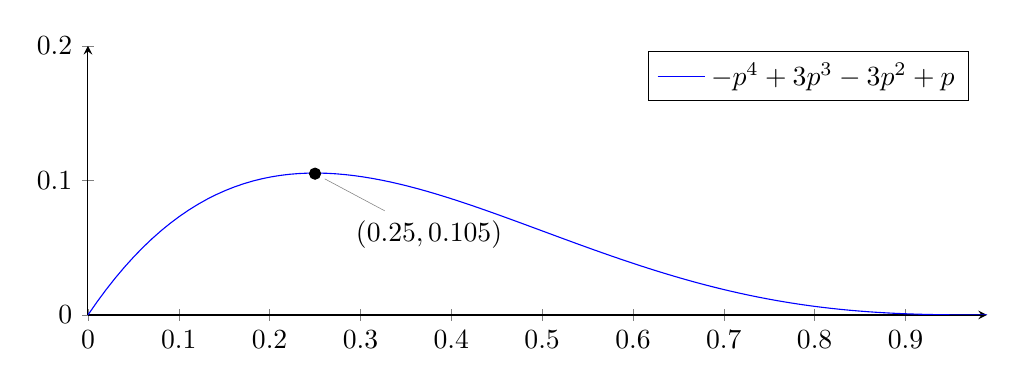
\begin{tikzpicture}
\begin{axis}[
    axis lines = left,
    ytick={0,0.1,0.2},
    ymin=0.0,ymax=0.2,
    xtick={0,0.1,0.2,0.3,0.4,0.5,0.6,0.7,0.8,0.9,1},
    height=5cm,
    width=13cm,
]

%Here the blue parabola is defined
\addplot [
    domain=0:1, 
    samples=100, 
    color=blue,
    ]
    {-x^4 + 3*x^3 -3*x^2 +x};
\addlegendentry{\(-p^4+3p^3-3p^2+p\)}

%Two dots are defined
\addplot[mark=*] coordinates {(0.25,0.105)} node[pin=310:{$(0.25,0.105)$}]{} ;

\end{axis}
\end{tikzpicture}
\end{center}
\\
From the graph, we can see that the vertex of the equation is $(0.25,0.105)$, which means that the biggest difference occurs when $p=0.25$ and the expected value of the two models differ by 0.148 tests.
\subsection{General term of the Worse Case}
As the method mentioned above, we are considering if the first grouping test is positive, the samples had to be retested individually. We did not include the special case, and in fact this make our calculation much easier. As the inflection rate is $p$ and the rate of not inflected is $(1-p)$, we know that all the combinations of the possibilities can be found with $(p+(1-p))^n$. Which is not useful then as we need to locate the special case. As we are not considering it, with less complexity, we can modify a general term to find out $T(p)$ for any group size $n$ by following steps.
\\
\\
Expanding $(p+(1-p))^n$:
\\
\\
\begin{array}{l}
(p+(1-p))^n\\
=p^{n} +C_{1}^{n}  \cdot p^{n-1} \left ( 1-p \right ) +C_{2}^{n }  \cdot p^{n-2} \left ( 1-p \right )^{2} +\dots +C_{G-1}^{n}  \cdot p^{n-\left ( n-1 \right ) } \left ( 1-p \right )^{n-1} +\left ( 1-p \right ) ^{n}\\
\end{array}
\\
\\
\\
By the General Term of Binomial Theorem, $(p+(1-p))^n$ can be expanded as above.
\\
\\
As we know that if there is at least one people inflected in the group, the number of test needed for the whole group is $(n+1)$ and if nobody was inflected in the group, only 1 test will be used. To find out T(p), we can multiply 1 to $(1-p)^n$ and multiply $(n+1)$ to all the terms remaining, such that the general term of expecting number of tests can be given out by:
\\
\\
\begin{array}{l}
T(p)=\left ( n+1 \right ) \left [ p^{n} +C_{1}^{n }  \cdot p^{n-1} \left ( 1-p \right ) +C_{2}^{n }  \cdot p^{n-2} \left ( 1-p \right )^{2} +\dots +C_{n-1}^{n }  \cdot p^{n-\left ( n-1 \right ) } \left ( 1-p \right )^{n-1} \right ]\\+\left 1( 1-p \right ) ^{n}
\end{array}
\\
\\
\\
By this general term, we don't need to count the combinations one by one like in the past, which dramatically increased the efficiency. Also, with less complexity, we can develop a program using Python and MATLAB easily to generate the equation of the expected value T(p) and find out the range of p $(p<)$ of any group size n . We also included the results when n = 2 to 100 from our calculation. \textbf{[Appendix 9.1]}

\subsection{Results}
The ideal sample results is summarized on the following table:
\\
\\
\begin{tabular}{p{5.25cm}p{5.25cm}p{6cm}}
\toprule
\textbf{Group size}&\textbf{Coordinate}&\textbf{Probability required}\\
\toprule
2&$(0.382,2)$&$p<0.382$\\
\midrule
3&$(0.343,3)$&$p<0.343$\\
\midrule
4&$(0.312,4)$&$p<0.312$\\
\bottomrule
\end{tabular}
\\
\\
\\
Observing the pattern, we found that the requirement of the infection rate $p$ increases as the groups size increases for the ideal solution.
\\
\\
The worse case results is summarized on the following table:
\\
\\
\begin{tabular}{p{5.25cm}p{5.25cm}p{6cm}}
\toprule
\textbf{Group size}&\textbf{Coordinate}&\textbf{Probability required}\\
\toprule
2&$(0.293,2)$&$p<0.293$\\
\midrule
3&$(0.306,3)$&$p<0.306$\\
\midrule
4&$(0.293,4)$&$p<0.293$\\
\bottomrule
\end{tabular}
\\
\\
\\
Observing the pattern, we found that the requirement of the infection rate $p$ is the same when sample size equal to 2 and 4 for the ideal solution. As we also calculated the range of $p$ for the worse case by program, from the data we get, we found that 3 have the highest comparability of range of $p$. Similar the ideal solution, the requirement of the infection rate $p$ increases as the groups size increases for the ideal solution after 4.\textbf{[Appendix 9.1]}
\\
\\
The difference results is summarized on the following table:
\\
\\
\begin{tabular}{p{3cm}p{3.5cm}p{3.5cm}p{6cm}}
\toprule
\textbf{Group size}&\textbf{Vertex}&\textbf{Inflection rate}&\textbf{Corresponding value of tests}\\
\toprule
2&$(0.5,0.25)$&0.5&0.25\\
\midrule
3&$(0.333,0.148)$&0.333&0.148\\
\midrule
4&$(0.25,0.105)$&0.25&0.105\\
\bottomrule
\end{tabular}
\\
\\
\\
Observing the pattern, it seems that the tests differ went smaller and smaller while the group size increases. This reasonable as the special case will always be 1 but the combinations of the group size is always increasing, the weight of the special case will become smaller and smaller as the group size increases. 

\subsection{Summary}
\begin{enumerate}
  \item We successfully build the simplest from of our model when the group size is equal to 2, 3 and 4, considered different situations and analyzed the result.
  \item From the data calculated, we discovered some interesting patterns:
  \begin{enumerate}
     \item In ideal solution, the requirement of the infection rate $p$ increases (must be lower) as the groups size increases. The worse case solution can get the same conclusion after the group size is greater than 4.
     \item The difference of expected value of test between the ideal test and the worse case went smaller and smaller while the group size increases.
    \end{enumerate}
  \item We also discovered some disadvantages of our model: 
  \begin{enumerate}
     \item We need to calculate the expected value for every group size if we need to compare the efficiency of different group sizes.
     \item As we can only find the range of $p$, we cannot find the maximum group size for a certain inflection rate $p$ by this method easily without advanced analysis.
    \end{enumerate}
\end{enumerate}